\documentclass{article}
\usepackage [T2A] {fontenc}
\usepackage[utf8]{inputenc}
\usepackage[russian,english]{babel}
\usepackage{amsmath,amssymb}
\usepackage[pdftex]{graphicx}
\begin{document}
А. Т. Улимаева
\\(г. Уфа)
\\РЕШЕНИЕ ЗАДАЧ НА НАХОЖДЕНИЕ НАИБОЛЬШИХ И НАИМЕНЬШИХ ЗНАЧЕНИЙ ФУНКЦИЙ
\\Опыт нашей работы в школах Башкирской АССР показал, что при организации повторения учебного материла в Х классе целесообразно рассматривать задачи на нахождение наибольших и наименьших значений функций, причем использовать при их решении наряду с аппаратом производной и другие способы. Это способствуют активизации мыслительной деятельности учащихся, вызывает у них интерес к решению задач и к изучению математики в целом.
\\Приведем пример решения одной такой задачи:
\\Требуется оградить прямоугольный участок земли площадью $a^2$. Определите оптимальные размеры участка, при которых затраты на ограду будут наименьшими (предполагается, что стоимость ограды пропорционально ее длине с коэффициентом $k>0$).
\\Решение. I способ. Найдем прямоугольник площади $a^2$, у которого периметр наименьший. Пусть $x>0$ -- длина стороны прямоугольника, тогда длина смежной с ней стороны равна $\frac{a^2}{x}$. Периметр прямоугольника $P(x)=2(x+\frac{a^2}{x})$.
\\Найдем наименьшее значение $P(x)$, применяя производную:
$$P'(x)=2(1-\frac{a^2}{x^2}), x\in]0;+\infty[$$
\\Определим критические точки функции:
$$(2(1-\frac{a^2}{x^2})=0)\Leftrightarrow(x=a\mbox{ или }x=-a)$$
\\так как $a>0$, то $x=a\in]0,+\infty[$.
\\Найдем следующие значения функции $P'(x)$:
$$P'(\frac{a}{2})=2(1-\frac{4a^2}{a^2})=-6<0$$
$$P'(2a)=2(1-\frac{a^2}{4a^2})=\frac{3}{2}>0$$
\\Следовательно, $\min\limits_{]0;+\infty[}P(x)=4a$ при $x=a$.
\\Длина другой стороны прямоугольника также равна $a$.
\\Из условия задачи известно, что стоимость изгороди $N(x)$ пропорциональна ее длине с коэффициентом $k>0:N(x)=k\cdot P(x)$. Следовательно $N(x)$ получит наименьшее значение, откуда 
$$N_{opt}(x)=\min\limits_{]0;+\infty[}N(x)=k\cdot4a\mbox{ при }x=a$$
\\Итак, чтобы оптимизировать стоимость изгороди, целесообразно выбрать участок квадратной формы.
\\II способ. Замечая, что $P(x)=2(x+\frac{a^2}{x})=2((\sqrt{x})^2-2\sqrt{x}\frac{a}{\sqrt{x}}+\frac{a^2}{(\sqrt{x})^2})+4a=2(\sqrt{x}-\frac{a}{\sqrt{x}})^2+4a$, где $x\in]0;+\infty[$, заключаем, что $\min\limits_{]0;+\infty[}P(x)=4a$ при $x=a$:
$$((\sqrt{x}-\frac{a}{\sqrt{x}})^2=0)\Rightarrow(\sqrt{x}=\frac{a}{\sqrt{x}})\Rightarrow(x=a)$$
\\III способ. Обозначим полупериметр прямоугольника $p(x)$. Пусть x -- длина одной из его сторон, тогда длина смежной с ней стороны равна $p-x(0\leqslant x\leqslant p)$. Площадь прямоугольника $a^2=x(p-x)$;
$$(x^2+a^2-px=0)\Leftrightarrow((x-a)^2+x(2a-p)=0$$
\\Последнее равенство истинно лишь при $2a-p\leqslant0$, т. е. при $p\geqslant2a$. Следовательно, наименьшее значение полупериметра равно 2a.
\\Подставляя в уравнение $x^2+a^2-px=0$ наименьшее значение $p$, получим уравнение $x^2-2a+a^2=0$, откуда $x=a$.
\\VI способ. Обозначим длины смежных сторон прямоугольника через $x$ и $y$, а его полупериметр через p. Тогда $xy=a^2$.
\\Чтобы найти наименьшее значение периметра прямоугольника площади $a^2$, воспользуемся известным тождеством: $(x+y)^2=(x-y)^2+4xy$. Заменив в нем произведение $xy$ на равное ему значение $a^2$, получим равенство
$$(x+y)^2=(x-y)^2+4a^2$$
\\Из этого равенства видно, что выражение $(x+y)^2=p^2$ получит наименьшее значение при $x-y=0$, т. е. при $x=y$. Полупериметр $p=x+y$ достигает своего наименьшего значения при $x=y=a$, при этом $P=4a$. 
\\V способ. По условию $xy=a^2$, где $x$ и $y$ -- длины смежных сторон прямоугольника.
\\Предположим, что $x\neq y$, пусть, например, $x=a+b(b>0)$, тогда 
$$y=\frac{a^2}{a+b}>\frac{a^2-b^2}{a+b}=a-b$$
\\Значит, $x+y>a+b+a-b=2a$.
\\Пусть теперь $x=y=a$. В этом случае $x+y=2a$.
\\Имеем: $x+y\geqslant2a$, откуда следует, что наименьшее значение периметра прямоугольника равно $4a$ и достигается оно при $x=y=a$
\\VI способ. К решению задачи можно применить также геометрические построения. В условии задачи дано: $xy=a^2$, где $x$ и $y$ -- длины смежных сторон прямоугольника.
\\При $x=y=a(a>0)$ получаем $x+y=2a$. Построим окружность с центром в точке $O$ радиуса $|AO|=a$. Имеем: $|AB|=|AO|+|OB|=x+y=2a$ (см. рис.).
\\
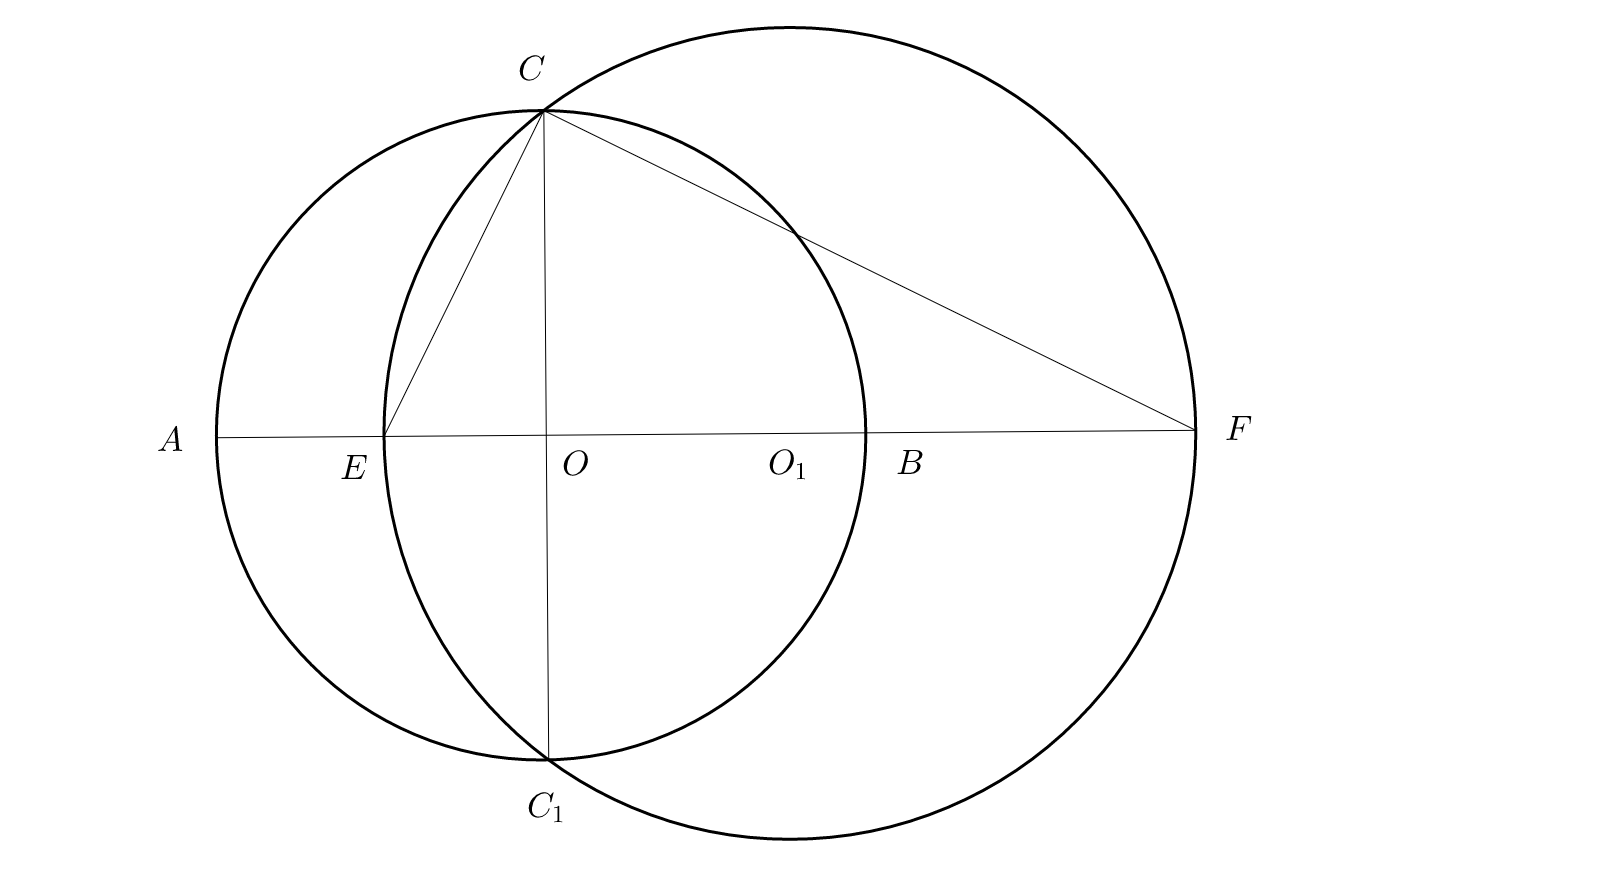
\includegraphics[scale=0.25]{circle.png}
\\Пусть $x\neq y$. Построим на том же рисунке окружность с центром в точке $O_1$ и радиусом, равным длине отрезка $O_1F$, так, чтобы $|EO|\cdot|OF|=a^2$. Тогда $|EO|+|OF|=|EF|$, где $|EO|=x$, $|OF|=y$.
\\Рассматривая рисунок, замечаем, что $|EF|>2a$, так как $|EF|$ -- длина диаметра, а $2a$ -- длина хорды $CC_1$ окружности $(O_1,|O_1F|)$. Таким образом получаем, что $x+y\geqslant2a$, причем $x+y=2a$ при $x=y=a$.
\\Т. П. Григорьева
\\(г. Горький)
\\К ИЗУЧЕНИЮ СКАЛЯРНОГО ПРОИЗВЕДЕНИЯ ВЕКТОРОВ
\\Доказательство распределительного свойства скалярного умножения векторов представляет трудности как в методическом, так и в математическом плане. В учебном пособии "Геометрия 9" ($\S$, с. 59) приведено доказательство этого свойства векторов. Существуют и другие доказательства (см.: Скопец З. А. О распределительном свойстве скалярного произведения векторов. --Математика в школе, 1965, № 6, с. 26; Скопец З. А. и др. Скалярное произведение двух векторов. --Математика в школе, 1968, № 6, с. 8; Скопец З. А. Соотношение Лейбница и распределительное свойство скалярного произведения векторов. --Квант, 1972, № 6, с. 22). Однако названные доказательства либо слишком алгебраичны, либо громоздки. Приведем новое доказательство, навеянное статьей З. А. Скопеца, опубликованной в № 6 журнала "Математика в школе" за 1965 г., которое, нам кажется, имеет преимущества по сравнению с указанными.
\\Предварительно с учащимися нужно рассмотреть метрическое свойство параллелограмма: сумма квадратов длин диагоналей параллелограмма равна сумме квадратов длин диагоналей параллелограмма равна сумме квадратов длин его сторон, т. е.
\begin{equation} \label{E1}
d_1^2+d_2^2=2a^2+2b^2.
\end{equation}
Доказательство этого свойства следует из равенств
\begin{equation} \label{E2}
(\overrightarrow{a}-\overrightarrow{b})^2=\overrightarrow{a^2}-2\overrightarrow{a}\cdot\overrightarrow{b}+\overrightarrow{b^2}
\end{equation}
и
\begin{equation} \label{E3}
(\overrightarrow{a}+\overrightarrow{b})^2=\overrightarrow{a^2}+2\overrightarrow{a}\cdot\overrightarrow{b}+\overrightarrow{b^2}
\end{equation}
и не представляет трудностей для учащихся.
\\Заметим, что метрическое соотношение \eqref{E1} может быть доказано ранее, в VIII классе, с помощью теоремы косинусов и применяется при решении других задач.
\\Перейдем теперь к доказательству распределительного свойства скалярного умножения векторов.
\\От точки $O$ отложим векторы $\overrightarrow{OA}=\overrightarrow{a},\overrightarrow{OB}=\overrightarrow{b},\overrightarrow{OC}=\overrightarrow{c}$.
\\
%
%
%картинка
%
%
\begin{center}
(Рис. 1)
\end{center}
а) Пусть точки $A$, $B$, $C$ не принадлежат одной прямой (рис. 1). Достроим треугольник $ABC$ до параллелограмма $ABCD$. Тогда $\overrightarrow{AB}=\overrightarrow{b}-\overrightarrow{a}, \overrightarrow{AC}=\overrightarrow{c}-\overrightarrow{a}, \overrightarrow{BC}=\overrightarrow{c}-\overrightarrow{b}$. Нетрудно видеть, что $\overrightarrow{a}+\overrightarrow{d}=\overrightarrow{b}+\overrightarrow{c}$, где $\overrightarrow{d}=\overrightarrow{OD}$, откуда $\overrightarrow{d}=\overrightarrow{b}+\overrightarrow{c}-\overrightarrow{a}, \overrightarrow{AD}=\overrightarrow{b}+\overrightarrow{c}-2\overrightarrow{a}$. Согласно \eqref{E1} запишем
$$2|AB|^2+2|AC|^2=|AD|^2+|BC|^2$$
или
$$2(\overrightarrow{b}-\overrightarrow{a})^2+2(\overrightarrow{c}-\overrightarrow{a})^2=((\overrightarrow{b}+\overrightarrow{c})-2\overrightarrow{a})^2+(\overrightarrow{c}-\overrightarrow{b})^2$$
После раскрытия скобок, основанных на равенствах \eqref{E2} и \eqref{E3}, получаем
$$\overrightarrow{b}\cdot\overrightarrow{a}+\overrightarrow{c}\cdot\overrightarrow{a}=(\overrightarrow{b}+\overrightarrow{c})\cdot\overrightarrow{a}$$
Отметим, что рассмотренное доказательство справедливо как для компланарных так и для некопланарных векторов.
\\Для полноты изложения рассмотрим два частных случая.
\\б) Пусть точки $A$, $B$, $C$ принадлежат одной прямой (рис. 2). Тогда введем вектор $k\overrightarrow{a}$, где $k\neq1,k\neq=$. Согласно случаю а) имеем:
$$k\overrightarrow{a}\cdot(\overrightarrow{b}+\overrightarrow{c})=(k\overrightarrow{a})\cdot\overrightarrow{b}+(k\overrightarrow{a})\cdot\overrightarrow{c}$$
или
$$k(\overrightarrow{a}\cdot(\overrightarrow{b}+\overrightarrow{c}))=k(\overrightarrow{a}\cdot\overrightarrow{b})+k(\overrightarrow{a}\cdot\overrightarrow{c})$$
После сокращения на $k$ получаем требуемое равенство.
\\
%
%
%картинка
%
%
\\в) Пусть векторы $\overrightarrow{a},\overrightarrow{b},\overrightarrow{c}$ коллинеарны. Тогда $\overrightarrow{a}=\alpha\overrightarrow{e}$. $\overrightarrow{b}=\beta\overrightarrow{e},\overrightarrow{c}=\gamma\overrightarrow{e}$, где $|\overrightarrow{e}|=1$. Отсюда следует:
\begin{equation}\label{E4}
\overrightarrow{a}\cdot(\overrightarrow{b}+\overrightarrow{c})=\alpha\overrightarrow{e}\cdot(\beta\overrightarrow{e}+\gamma\overrightarrow{e})=\alpha\overrightarrow{e}\cdot(\beta+\gamma)\overrightarrow{e}=\alpha(\beta+\gamma)=\alpha\beta+\alpha\gamma
\end{equation}
С другой стороны,
\begin{equation}\label{E5}
\overrightarrow{a}\cdot\overrightarrow{b}+\overrightarrow{a}\cdot\overrightarrow{c}=(\alpha\overrightarrow{e})\cdot(\beta\overrightarrow{e})+(\alpha\overrightarrow{e})\cdot(\gamma\overrightarrow{e})=\alpha\beta+\alpha\gamma
\end{equation}
Сравнивая правые части равенств \eqref{E4} и \eqref{E5}, получаем истинность распределительного закона скалярного умножения векторов и для этого случая.
\\На уроке достаточно ограничиться общим случаем. Случаи б) и в) можно предложить либо в качестве упражнений, либо при повторении, либо сообщить учащимся лишь идею доказательства.
\\Приведем пример применения распределительного свойства скалярного умножения векторов.
\\Задача. Даны четыре точки $A,B,C,D$. Известны расстояния между этими точками: $|DA|=a,|DB|=b,|DC|=c,|AB|=a_1,|BC|=a_1,|AC|=b_1$. Найдите расстояние от одной из этих точек до центроида \footnote[1]{Центроидом трех точек $P,Q,R$ называется такая точка $G$, что $$\overrightarrow{OG}=\frac{1}{3}(\overrightarrow{OP}+\overrightarrow{OQ}+\overrightarrow{OR})$$} оставшихся трех точек.
\\Решение. Пусть требуется найти расстояние от точки $D$ до центроида $G$ точек $A,B,C$ (рис. 3). Введем векторы: $\overrightarrow{DA}=\overrightarrow{a},\overrightarrow{DB}=\overrightarrow{b},DC=\overrightarrow{c}$. Тогда
$$\overrightarrow{DG}=\frac{1}{3}(\overrightarrow{a}+\overrightarrow{b}+\overrightarrow{c})$$
отсюда 
$$\overrightarrow{DG}^2=\frac{1}{9}((\overrightarrow{a}+\overrightarrow{b})+\overrightarrow{c})^2=\frac{1}{9}((\overrightarrow{a}+\overrightarrow{b})^2+2(\overrightarrow{a}+\overrightarrow{b})\cdot\overrightarrow{c}+\overrightarrow{c}^2)$$
\\Согласно распределенному свойству скалярного умножения векторов имеем 
$$\overrightarrow{DG}^2=\frac{1}{9}(\overrightarrow{a}^2+\overrightarrow{b}^2+\overrightarrow{c}^2+2\overrightarrow{a}\cdot\overrightarrow{b}+2\overrightarrow{b}\cdot\overrightarrow{c}+2\overrightarrow{c}\cdot\overrightarrow{a})$$
\\Но
$$\overrightarrow{a}\cdot\overrightarrow{b}=\frac{\overrightarrow{OA}^2+\overrightarrow{OB}^2-\overrightarrow{AB}^2}{2}=\frac{a^2+b^2-c_1^2}{2}$$
$$\overrightarrow{b}\cdot\overrightarrow{c}=\frac{\overrightarrow{OB}^2+\overrightarrow{OC}^2-\overrightarrow{BC}^2}{2}=\frac{b^2+c^2-a_1^2}{2}$$
$$\overrightarrow{c}\cdot\overrightarrow{a}=\frac{\overrightarrow{OC}^2+\overrightarrow{OA}^2-\overrightarrow{AC}^2}{2}=\frac{c^2+a^2-b_1^2}{2}$$
\\поэтому
\begin{equation}\label{E6}
|DG|^2=\frac{1}{3}(a^2+b^2+c^2)-\frac{1}{9}(a_1^2+b_1^2+c_1^2)
\end{equation}
Отметим, что если точки $A,B,C,D$ являются вершинами тетраэдра $ABCD$, то квадрат длины отрезка $|DG|$ вычисляется по формуле \eqref{E6}.
\\Решая эту задачу, мы попутно вывели формулу скалярного квадрата суммы трех векторов:
$$(\overrightarrow{a}+\overrightarrow{b}+\overrightarrow{c})^2=\overrightarrow{a}^2+\overrightarrow{b}^2+\overrightarrow{c}^2+2\overrightarrow{a}\cdot\overrightarrow{b}+2\overrightarrow{b}\cdot\overrightarrow{c}+2\overrightarrow{c}\cdot\overrightarrow{a}$$
Эта формула часто применяется при решении задач.
\\Материал, рассмотренный в статье может быть использован учителем на уроках геометрии как при непосредственном изучении материала, так и при его повторении, а также на внеклассных занятиях.
\end{document}
